% Indicate the main file. Must go at the beginning of the file.
% !TEX root = ../main.tex

%%%%%%%%%%%%%%%%%%%%%%%%%%%%%%%%%%%%%%%%%%%%%%%%%%%%%%%%%%%%%%%%%%%%%%%%%%%%%%%%
% 04_discussion
%%%%%%%%%%%%%%%%%%%%%%%%%%%%%%%%%%%%%%%%%%%%%%%%%%%%%%%%%%%%%%%%%%%%%%%%%%%%%%%%


\section{Discussion}
\label{discussion}

\subsection{Detection}
The detection process substantially influenced the dataset composition, particularly on the sequence level for the \texttt{mustela\_erminea} category.
This category experienced higher data loss, likely due to the relative size of the species---it is much larger than the other species captured by these MammaliaBox camera traps.
This larger size may have resulted in more frequent bad shots due to closeness to the camera or the speed at which they pass through the box---many images showed only the tip of the animal's tail disappearing out of the box.
The difficulty of properly detecting stoats using camera traps is a known issue examined, for example, by \textcite{crooseAssessingDetectabilityIrish2022}.
Another interesting observation was that the white-fur individuals were more often not detected than the brown-fur individuals.
An explanation has yet to be found for why this was only the case on the sequence level, where the \texttt{mustela\_erminea} category was disproportionately affected.
On the image level, the \texttt{soricidae} category was the most affected, with \(23\%\) of the images lost but only \(1\%\) of the sequences.

Visual inspection revealed a mixture of exemplary BBox detections alongside notable inaccuracies, such as missed detections in images with obstructions or partial visibility of animals.
Looking through misclassified images with high confidence values revealed some interesting insights.
One was that quite a few false positive detections were made, leading to surprisingly high-confidence classifications.
Some of these images were empty or contained no animal at all, as shown in \autoref{fig:false_positive_dt}, which includes examples where plant parts were misdetected, animals appeared in very dark areas, or very small, not clearly visible objects were present.
Another interesting finding was that quite a few of the images contained a snail in the highest-confidence BBox---refer to \autoref{fig:false_class_snails} for a hand-picked selection of these examples.
These misclassifications highlight the need for enhanced object discrimination capabilities or the introduction of an additional class for non-target species.

The dilemma of not missing potentially relevant detections while also not polluting the dataset with image noise remains a challenge.
Simply lowering the detection threshold to reduce missed animals is not a viable solution.
As \textcite{leornaHumanVsMachine2022} showed, reducing the \ac{MD} confidence threshold substantially increased recall, but at the cost of a profound increase in false positives, such as empty frames or vegetation.
This calls for a more sophisticated approach to reduce missed detections while maintaining a clean dataset.

\begin{figure}[ht]
\centering
\includegraphics[width=\textwidth]{figures/false_positive_dt.pdf}
\caption{Examples of false positives with high classification confidence but no animal present.}
\label{fig:false_positive_dt}
\end{figure}

\begin{figure}[ht]
\centering
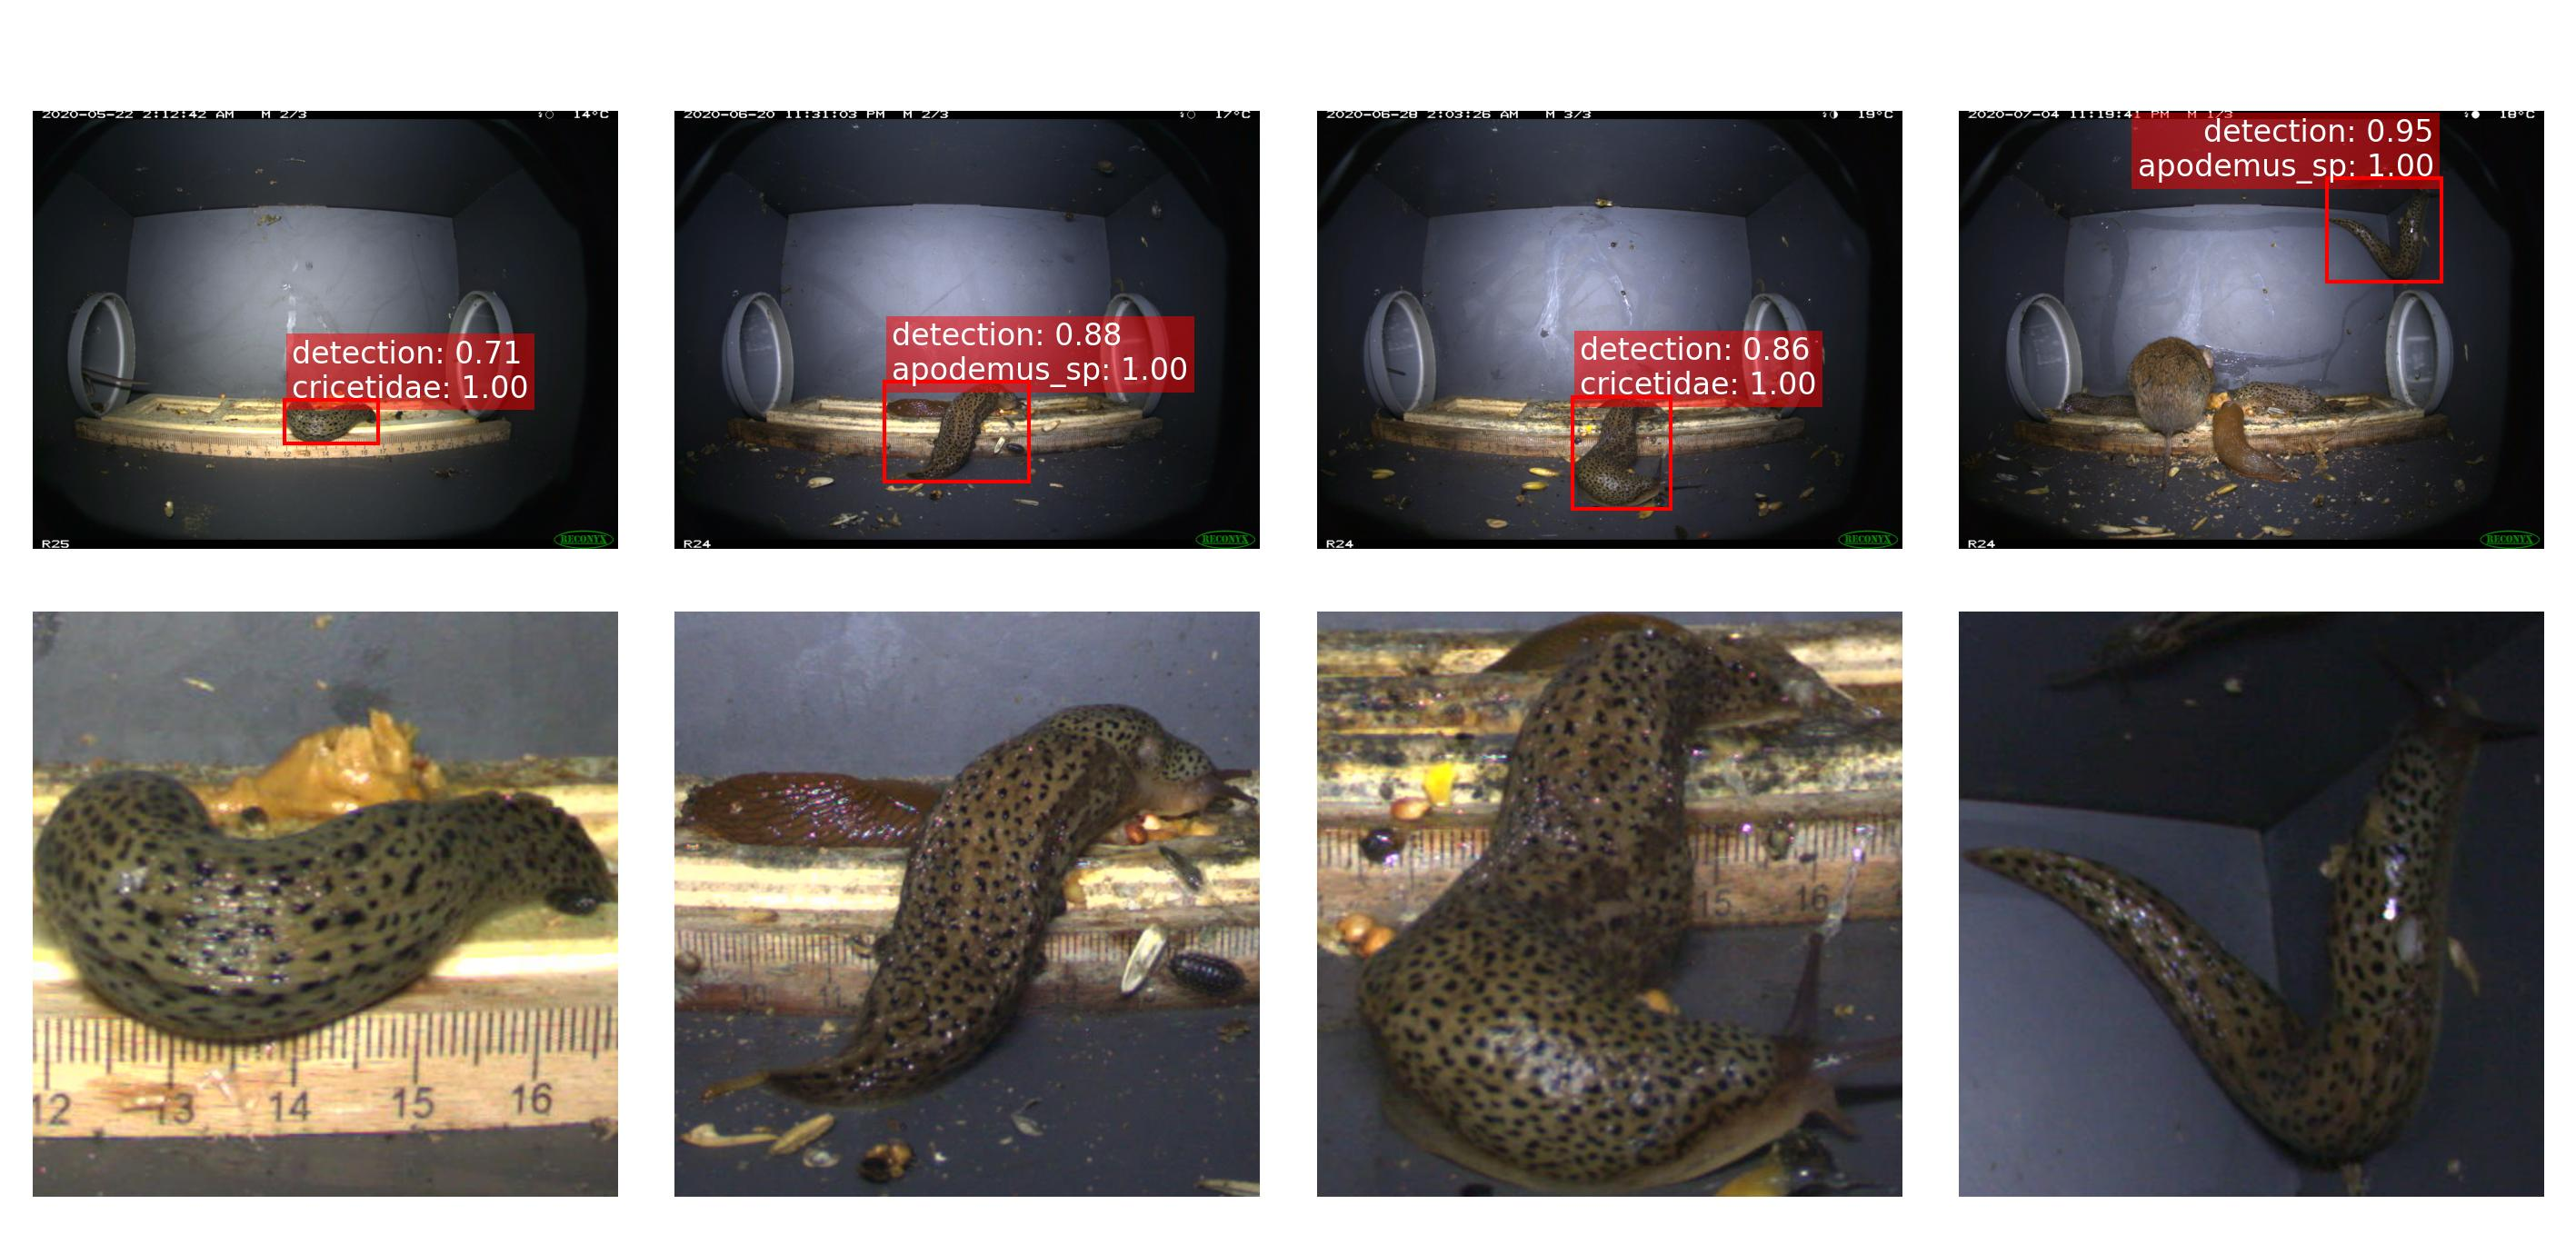
\includegraphics[width=\textwidth]{figures/false_class_snails.pdf}
\caption{Hand-picked selection of misclassified images where a snail appears in the highest-confidence BBox.}
\label{fig:false_class_snails}
\end{figure}

\subsection{Model Performance}
All tested models achieved high performance in image classification tasks, demonstrating their suitability for automating small mammal identification.
Pretrained models slightly outperformed those trained from scratch, underscoring the value of transfer learning.
The slightly better balanced accuracy of pretrained models is just one of the benefits of using pretrained models, as they also require less training time and computational resources---and hence less energy---and could potentially be trained with less data.
There are various studies exploring or applying transfer learning to camera trap images, underscoring its potential \autocite{stancicClassificationEfficiencyPreTrained2022,hopkinsDetectingMonitoringRodents2024,doanWildlifeSpeciesClassification2024,rameshExploringGeneralizabilityTransfer2025,beeryRecognitionTerraIncognita2018}.\todo{(What's the difference? Delete one?)}

Interestingly, the smaller the models, the better they performed on the image-level classification task, highlighting the fact that bigger is not always better.
Smaller models, if complex enough for the task, are always preferable since they require fewer computational resources and are faster to train.
The proper scaling of a model is an important aspect of model selection, as emphasized, for example, by \textcite{tanEfficientNetRethinkingModel2019}.
Examining \autoref{fig:bal_acc_img} again, one could speculate about a trend for smaller models to perform more consistently across folds when trained from scratch---but for some reason, this is not the case for the EfficientNet-B0 model.
The observations from this study suggest that smaller, computationally efficient models are sufficient and therefore preferable for the classification tasks at hand.


\subsection{Best Model Architecture}
The pretrained EfficientNet-B0 emerged as the best-performing architecture, achieving the highest \ac{BA}.
\autoref{fig:training_metrics_best_model} shows the validation metrics for each cross-validation fold across all epochs; note that accuracy is reported in the figure instead of \ac{BA}.
For all folds, the best version, defined by the lowest validation loss, occurred within the first few epochs, while accuracy continued to improve.
While an increase in accuracy indicates more correct predictions, the loss can still worsen because it also penalizes correct predictions made with low confidence and incorrect predictions made with high confidence.

Since the training dataset was quite large, contained only four classes and was intensively vetted using the \ac{MD}, the model was able to learn the task quite quickly.
The initial supposition that a higher detection confidence would lead to a higher classification confidence could not be confirmed by the Spearman's rank correlation coefficient.
It even suggested that the correlation is stronger for incorrect classifications.
Examining \autoref{fig:pred_conf_hexbin}, which shows the relationship between detection confidence and classification confidence, reveals that classification confidence is generally very high---across all detection confidence values and even for incorrect classifications.
There seem to be more values located in the upper right corner, which would suggest that higher detection confidence leads to higher classification confidence.
However, since there are so many samples with classification confidence close to 1 across the range of detection confidence values, Spearman's rank may not be a good measure for this relationship.

The generally high classification confidence values could be explained by the model's architecture.
In the last layers of the model, the learned features are mapped to the four classes and then normalized so the values sum to one.
If the model is entirely confident that an input does not belong to the first three classes and assigns a very small value to the fourth class (e.g., \([0\;;\;0\;;\;0\;;\;10^{-5}]\)), this distribution will be normalized to \([0\;;\;0\;;\;0\;;\;1]\), resulting in a prediction for the fourth class with maximum confidence.
As shown by \textcite{hendrycksBaselineDetectingMisclassified2018}, softmax-based confidence scores often fail to meaningfully reflect true uncertainty, especially for \ac{OOD} inputs.
Therefore, this evaluation lacks meaningfulness.
It could be repeated using logits without normalization.
Nonetheless, the assumption that a non-target class would benefit the classification task remains valid.

\begin{figure}[ht]
\centering
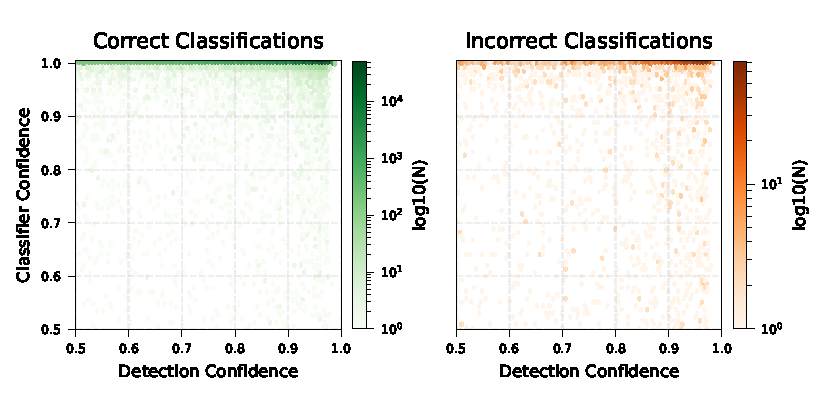
\includegraphics{figures/pred_conf_hexbin.pdf}
\caption{Hexbin plot of detection confidence vs. classification confidence for correct and incorrect predictions. Color scale indicates log$_{10}$-binned counts.}
\label{fig:pred_conf_hexbin}
\end{figure}

\subsection{Limitations}
The primary limitation of the current methodology is the absence of an explicit non-target class, forcing models into potentially incorrect predictions, particularly under \ac{OOD} conditions, exemplified by the snail misclassification issue shown in \autoref{fig:false_class_snails}.
Further, despite improvements, the \ac{MD} still misses a significant number of potentially relevant detections.
This limitation is particularly pronounced for rare species, where insufficient data reduces detection reliability.
The loss of sequences for the \texttt{mustela\_erminea} category, as shown in \autoref{tab:data_availability_after_md}, illustrates this issue.
Every sequence completely lost is a potentially missed sighting of a rare species, which could have provided valuable insights for conservation efforts.

The step of sequence classification is performed on the model's classification confidence values per class and image.
Since the information from the logits is heavily distorted by the normalization step, sequence classification does not yet reach its full potential.
This approach might need to be revisited to improve the reliability of sequence-level results.
The current approach also depends on manual preprocessing of the dataset to group the images into sequences---this process would benefit from automation.

Moreover, the current approach is heavily dependent on data availability.
Rare species inherently have fewer data points, constraining model training and potentially biasing predictions.
To include an additional class would require a sufficient number of samples to ensure reliable model performance.
Generally, data acquisition is the most resource-intensive part of most machine learning projects.

